% Created 2022-12-18 Sun 20:28
\documentclass[9pt, b5paper]{article}
\usepackage{xeCJK}
\usepackage{minted}
\usepackage[T1]{fontenc}
\usepackage[scaled]{beraserif}
\usepackage[scaled]{berasans}
\usepackage[scaled]{beramono}
\usepackage{graphicx}
\usepackage{xcolor}
\usepackage{multirow}
\usepackage{multicol}
\usepackage{float}
\usepackage{textcomp}
\usepackage{algorithm}
\usepackage{algorithmic}
\usepackage{latexsym}
\usepackage{natbib}
\usepackage{geometry}
\geometry{left=1.2cm,right=1.2cm,top=1.5cm,bottom=1.2cm}
\newminted{common-lisp}{fontsize=\footnotesize} 
\usepackage[xetex,colorlinks=true,CJKbookmarks=true,linkcolor=blue,urlcolor=blue,menucolor=blue]{hyperref}
\author{deepwaterooo}
\date{\today}
\title{Unity Export 导出到Android Studio再打包大致过程}
\hypersetup{
  pdfkeywords={},
  pdfsubject={},
  pdfcreator={Emacs 27.2 (Org mode 8.2.7c)}}
\begin{document}

\maketitle
\tableofcontents


\section{UnityPlayerActivity中onDestroy()时mUnityPlayer会杀死整个进程的问题[爱表哥,爱生活]}
\label{sec-1}

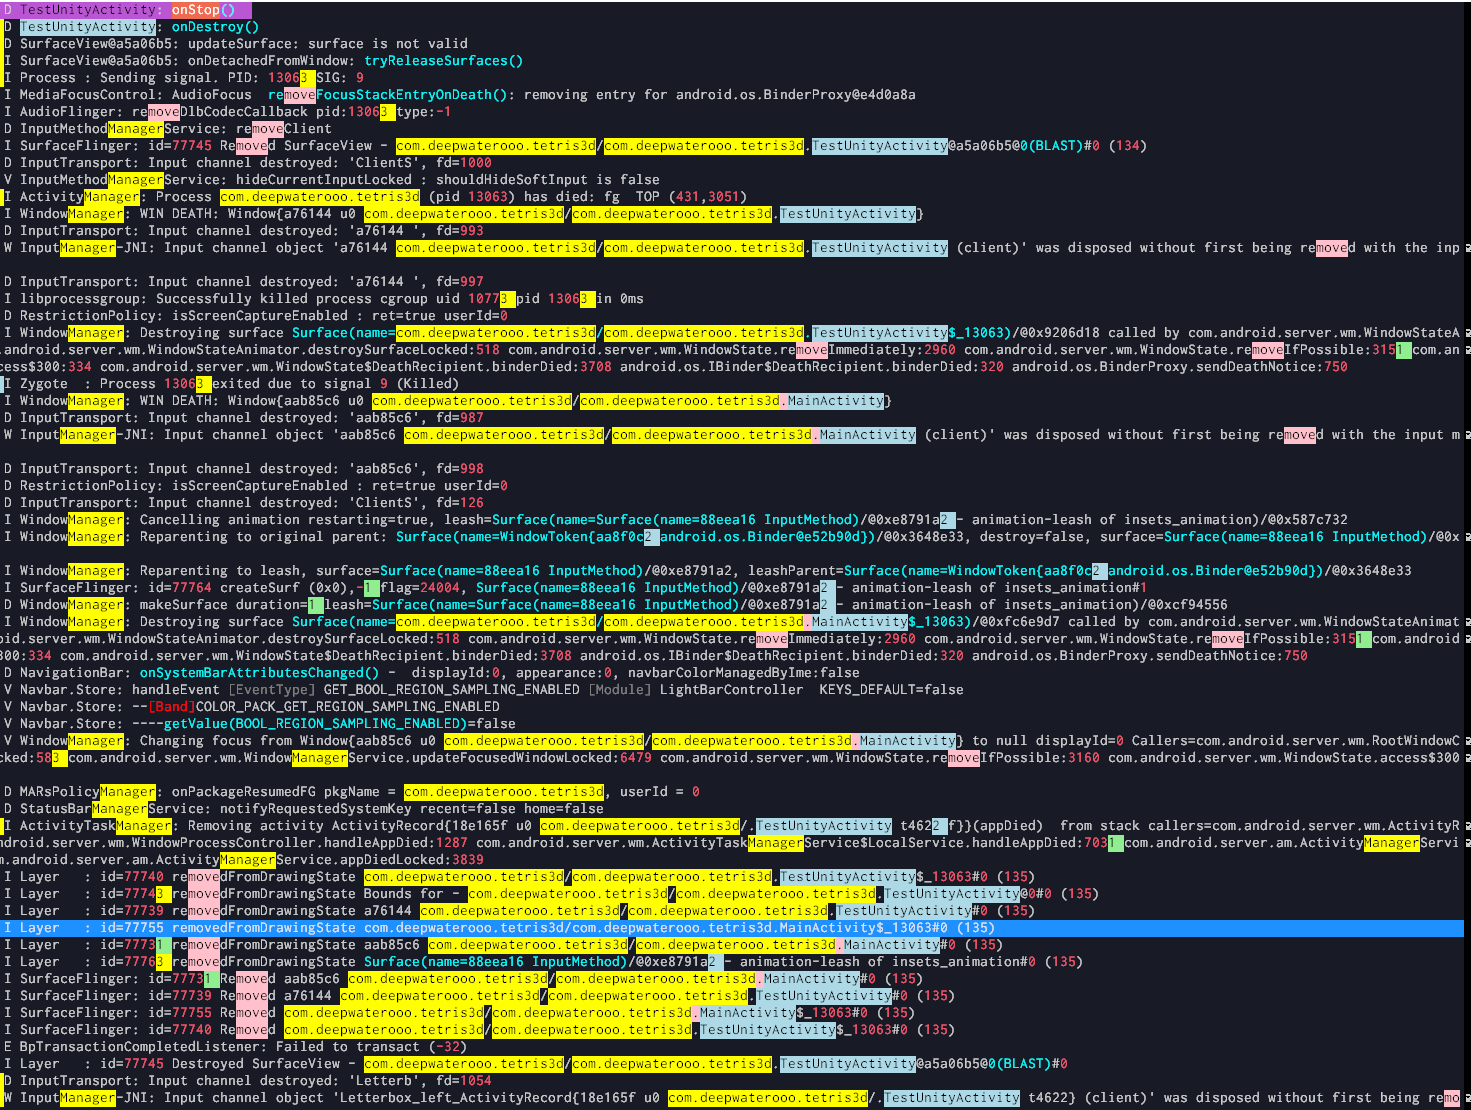
\includegraphics[width=.9\linewidth]{./pic/unityToAndroid_20221208_092915.png}
\begin{itemize}
\item 这里它就把想要启动的安卓MainActivity的视图也给销毁了
\end{itemize}
\subsection{相关部分的源码:}
\label{sec-1-1}
\subsubsection{UnityPlayerActivity}
\label{sec-1-1-1}
\begin{minted}[fontsize=\scriptsize,linenos=false]{cpp}
protected void onDestroy() {
    this.mUnityPlayer.quit(); // <<<<<<<<<<<<<<<<<<<< 
    super.onDestroy();
}
\end{minted}
\subsubsection{UnityPlayer}
\label{sec-1-1-2}
\begin{minted}[fontsize=\scriptsize,linenos=false]{cpp}
    protected void kill() {
        Process.killProcess(Process.myPid()); // <<<<<<<<<< 这是就把整个进程给杀死了
    }
    public void quit() {
        GoogleVrProxy var1;
        if ((var1 = GoogleVrApi.b()) != null) {
            GoogleVrApi.a();
            var1.b();
        }

        this.p = true;
        if (!this.e.e()) {
            this.pause();
        }

        this.a.a();

        try {
            this.a.join(4000L);
        } catch (InterruptedException var2) {
            this.a.interrupt();
        }

        if (this.g != null) {
            this.m.unregisterReceiver(this.g);
        }

        this.g = null;
        if (com.unity3d.player.l.c()) {
            this.removeAllViews();
        }

        this.kill(); // <<<<<<<<<<<<<<<<<<<< 
        g();
    }
\end{minted}

\subsection{解决办法: 网上搜索到几种解决方法,及其相关后续可能存在的问题}
\label{sec-1-2}
\subsubsection{自定义 UnityPlayer,绕过杀进程的部分}
\label{sec-1-2-1}
\begin{itemize}
\item \url{https://gameinstitute.qq.com/community/detail/129065}
\begin{minted}[fontsize=\scriptsize,linenos=false]{java}
/**
 * 主要是重写父类的{@link UnityPlayer#kill}方法,因为父类的做法太粗暴了,让Activity自己去finish即可
 */
public class MyUnityPlayer extends UnityPlayer {

    public MyUnityPlayer(ContextWrapper contextWrapper) {
        super(contextWrapper);
    }
    // * 不执行父类方法
    @Override
    protected void kill() {
        // super.kill();
    }
}
\end{minted}
\item Activity中这样使用:
\end{itemize}
\begin{minted}[fontsize=\scriptsize,linenos=false]{java}
protected UnityPlayer mUnityPlayer;

@Override
protected void onCreate(Bundle savedInstanceState) {
    requestWindowFeature(Window.FEATURE_NO_TITLE);
    super.onCreate(savedInstanceState);

    ActivityManager.putActivity(this);
    getWindow().setFormat(PixelFormat.RGBX_8888); // This makes xperia play happy

    // mUnityPlayer = new UnityPlayer(this); 
    mUnityPlayer = new MyUnityPlayer(this); // <<<<<<<<<<<<<<<<<<<< 
    setContentView(mUnityPlayer);
    mUnityPlayer.requestFocus();
}
\end{minted}
\subsubsection{因为还没有如此实现,不知道还会有哪些后续的问题}
\label{sec-1-2-2}
\begin{itemize}
\item \textbf{Note: 然而最近在使用上面重写后又出现问题了,会导致Unity的界面无法正常显示,就没有用了!}
\item 我因为还没有如此实现,不知道还会有哪些后续的问题
\item 其它网友提到过的还存在的问题包括: \textbf{[这些,需要用自己的游戏来验证一下]}
\begin{itemize}
\item 项目中最近在做一个 AR 扫行标(银行 Logo)抽奖的活动,动画模型依托 Unity 环境来展现的。Android 集成 Unity 很简单(比 iOS 方便太多),但是在使用过程中还是需要到一点小麻烦。
\item 需求中要求扫描页面可以反复进出,在 @Override protected void onDestroy () 生命周期的回调方法中需要调用 mUnityPlayer.quit(); 来达到退出 Unity 的目的。但是发现 mUnityPlayer.quit(); 方法会杀死当前进程,
\item 不调用 mUnityPlayer.quit(); 方法,控制台中又会提示一个服务没有被清理,会发生内存泄漏,
\item 网上的做法是集成 UnityPlayer 写一个新类,重写掉 kill() 方法,不杀死进程,但是 \textbf{实验了之后发现没有效果,依然会有内存泄漏的提示,虽然大部分机型可以正常使用,但是测试中小米和其他品牌的部分机型在反复进出几次 Unity 程序后,会闪退} 。 \textbf{[感觉这里的问题没有追查到底,是资源完全没能释放,还是部分释放了?对于出问题的手机型号,没有提供或作进一步的征查资源释放过程中的问题.如果我能拿到日志,会想到分析得再彻底一点儿]}
\end{itemize}
\item \textbf{自己的项目暂时只实现到这里,会留意是否会有后续问题,再考虑是否游戏端活动放独立进程}
\end{itemize}
\subsubsection{与上面第一种方法同理,接上面的(继上面两步之后),别人还使用过的方法包括:}
\label{sec-1-2-3}
\begin{itemize}
\item 原理同样是绕过unity游戏端的桥接类UnityPlayerActivity UnityPlayer中杀掉进程的这一步,只是是通过调用安卓端实现的方法来结束unity游戏端活动
\item 在unity中调用android接口返回上级activity
\end{itemize}
\begin{minted}[fontsize=\scriptsize,linenos=false]{csharp}
private static void BackToShelfFromAndroid() {
    using (AndroidJavaClass jc = new AndroidJavaClass("com.dps.core.UnityInterface")) {
        jc.CallStatic("backToShelf");
    }
}
\end{minted}
\begin{itemize}
\item 实现android接口:
\end{itemize}
\begin{minted}[fontsize=\scriptsize,linenos=false]{java}
public static void backToShelf() {
    Log.i("unity","finish unityPlayer ");
    UnityPlayer.currentActivity.finish(); // 这里就是正常安卓活动的finish()方法
}
\end{minted}
\subsubsection{另一种: 特制结束游戏端活动广播;调用安卓端活动以借其发送结束游戏端活动广播;安卓端特制类专门负责接收广播,并结束游戏端活动,感觉很绕,性能?}
\label{sec-1-2-4}
\begin{itemize}
\item 再看最后一个游戏端放独立进程的作比较,就会发现这里安卓端的发送广播与接收广播都是很绕的自找麻烦的浪费性能的过节,这里应该完全可以不用多一步广播的定义,注册发送与接收
\item 创建一个UnityReaderActivity继承UnityPlayerActivity,在此注册一个广播接收,接收到广播后finish此UnityReaderActivity。在onPause中用super.onDestroy()替换掉super.onPause()。
\end{itemize}
\begin{minted}[fontsize=\scriptsize,linenos=false]{java}
// 这个类只做一件事: 专门负责接收游戏端发送过来,要求结束游戏端活动的广播,接收后结束游戏端活动(绕过游戏端的杀进程)
public class UnityReaderActivity extends UnityPlayerActivity {
    // 自身的引用
    private BroadcastReceiver receiver;
 
    @Override
    protected void onCreate(Bundle savedInstanceState) {
        super.onCreate(savedInstanceState);
        registBroadcast();
    }
 
    // Pause Unity
    @Override
    protected void onPause() {
        if (receiver != null) {
            unregisterReceiver(receiver);
        }
        // super.onPause();
        super.onDestroy(); // <<<<<<<<<<<<<<<<<<<< 此处是关键: 生命周期调用的错位,仍然感觉狠粗暴,不优雅
    }
  
    private void registBroadcast() {
        receiver = new FinishUnityBroadcast();
        IntentFilter filter = new IntentFilter();
        filter.addAction("finishunity");
        registerReceiver(receiver, filter);
    }
 
    class FinishUnityBroadcast extends BroadcastReceiver {
        @Override
        public void onReceive(Context context, Intent intent) {
            finish();
        }
    }
}
\end{minted}
\begin{itemize}
\item 使用时调用UnityReaderActivity ,在AndroidManifest.xml中注册UnityReaderActivity
\end{itemize}
\begin{minted}[fontsize=\scriptsize,linenos=false]{xml}
<activity
    android:name=".UnityReaderActivity"
    android:configChanges="mcc|mnc|locale|touchscreen|keyboard|keyboardHidden|navigation|orientation|screenLayout|uiMode|screenSize|smallestScreenSize|fontScale|layoutDirection"
    android:hardwareAccelerated="true"
    android:label="@string/app_name"
    android:launchMode="singleTask"
    android:screenOrientation="portrait"
    android:windowSoftInputMode="adjustResize" >
  <meta-data
      android:name="unityplayer.UnityActivity"
      android:value="true" />
</activity>
\end{minted}
\begin{itemize}
\item 在unity中调用android接口发送广播结束UnityReaderActivity返回上级activity
\begin{itemize}
\item unity调用android接口:
\end{itemize}
\end{itemize}
\begin{minted}[fontsize=\scriptsize,linenos=false]{csharp}
private static void BackToShelfFromAndroid() {
    using (AndroidJavaClass jc = new AndroidJavaClass("com.dps.core.UnityInterface")) {
        jc.CallStatic("backToShelf");
    }
}
\end{minted}
\begin{itemize}
\item 实现android接口:
\end{itemize}
\begin{minted}[fontsize=\scriptsize,linenos=false]{java}
public static void backToShelf() {
    Log.i("unity","finish unityPlayer ");
    mContext.sendBroadcast(new Intent("finishunity"));
}
\end{minted}

\subsubsection{把UnityPlayerActivity放在独立的进程,也会带来后续多进程数据交互相关的问题?}
\label{sec-1-2-5}
\begin{itemize}
\item \url{https://www.cxyzjd.com/article/weixin_42123296/112024546}
\item 首先,把UnityPlayer所在的Activity放到一个新的进程里: 加入android:process=”:unity”
\end{itemize}
\begin{minted}[fontsize=\scriptsize,linenos=false]{xml}
<activity
    android:name=".UnityPlayerActivity"
    android:label="@string/app_name"
    android:launchMode="singleTask" 
    android:screenOrientation="landscape"

    android:process=":unity"

    android:theme="@android:style/Theme.NoTitleBar.Fullscreen"
    android:name="unityplayer.UnityActivity"
    android:value="true" />
\end{minted}
\begin{itemize}
\item 接下来,按照下面步骤进行:[这可以尝试作为另一种方法的实现,不是加法,是或者]
\begin{itemize}
\item 第一步,在activity里定义一个unityFinish方法。
\item 第二步,在unity脚本中调用activity里定义好的unityFinish方法。(如不知道怎么调用请移步到:Android 与 Unity 的交互) \textbf{[同上面的安卓端的广播定义注册发送与接收相比,省性能了]}
\item 第三步,activity的unityFinish方法里处理一些结束操作,最后调用Activity的finish()。 \textbf{[可以成功绕过那个杀死自己进程的步骤]}
\item 第四步,在activity的destroy方法里调用UnityPlayer的quit()。 \textbf{[在必要需要的进候,仍然进行了必要的资源释放,只是不知道能否在有限制时间里清理干净,还是说会自动延迟,或是程序员给足它时间清理干净呢?]}
\end{itemize}
\item 这样你需要进行结束要处理的事情放到了自己定义的方法里进行了处理,处理完后调用Activity的finish(),这样activity开始走自己结束的方法,在Activity的的destroy方法里调用super.onDestroy()之前调用mUnityPlayer.quit(),这个时候会先走UnityPlayer的quit()处理后事,这样即使把自己的宿主进程kill了,用户也感知不到了。
\item 缺点: \textbf{后面的四个步骤感觉逻辑还比较清淅,可是感觉作者可能也没能理解透彻,步骤有多余},当游戏端活动处于独立的进程,那杀进程就杀呀,它反正是在独立的进程,死了那个游戏端活动的进程,不影响其它安卓端进程呀,它的前后两部分其实应该可以独立到两种不同的实现方法里去的,而不是同时处理两种方法???
\item 独立进程可能带来的问题: \url{https://www.jianshu.com/p/046590c1e6b3}
\end{itemize}
\begin{minted}[fontsize=\scriptsize,linenos=false]{xml}
<activity
    android:name="cn.com.global_vision_ar.UnityPlayerActivity"
    android:screenOrientation="portrait"
    android:process=":unityAR"
</activity>
\end{minted}
\begin{itemize}
\item 这个办法解决了闪退问题,但是还没有结束,UnityPlayerActivity 中需要接收 AR 程序的回调方法,如:public void getGift() ,在这个方法中请求后台接口,发起抽奖。Unity 程序改成用新进程启动后,发起抽奖接口时,发生了会话丢失的情况(抽奖是需要登录的,后台会话是基于 Cookie 中的 JessionId)。我猜是因为不在同一个进程,Cookie 没有同步,导致送到后台的 JessionId 不一致(不是登录成功后返回的 JessionId)。
\item 解决办法是使用 Broadcast 跨进程通信,把抽奖的请求写在主进程,要抽奖时发起广播进行抽奖,抽奖结束后得到抽奖结果的数据,再通过广播的方式把数据传回 UnityPlayerActivity,使用 UnityPlayer.UnitySendMessage 方法通知 Unity 程序。
\end{itemize}

\section{安卓导.jar .aar进unity几个细巧点}
\label{sec-2}
\subsection{项目的build.grale}
\label{sec-2-1}
\begin{minted}[fontsize=\scriptsize,linenos=false]{groovy}
plugins {
    id 'com.android.library' // <<<<<<<<<<<<<<<<<<<< 可以直接把app 改成早类库就可以了,不同再导一个
}
android {
    namespace 'com.deepwaterooo.dwsdk' // <<<<<<<<<<<<<<<<<<<< 这个需要
    compileSdk 32
    defaultConfig {
        minSdk 25
        targetSdk 32
        versionCode 1
        versionName "1.0"
        testInstrumentationRunner "androidx.test.runner.AndroidJUnitRunner"
    }
    buildTypes {
        release {
            minifyEnabled false
            proguardFiles getDefaultProguardFile('proguard-android-optimize.txt'), 'proguard-rules.pro'
        }
    }
    compileOptions {
        sourceCompatibility JavaVersion.VERSION_1_8
        targetCompatibility JavaVersion.VERSION_1_8
    }
}
dependencies {
    compileOnly files('libs\\classes.jar') // <<<<<<<<<<<<<<<<<<<< compileOnly Unity里的这些类是分Mono il2cpp的,要区分
    implementation 'androidx.appcompat:appcompat:1.5.1'
    implementation 'com.google.android.material:material:1.7.0'
    implementation 'androidx.constraintlayout:constraintlayout:2.1.4'
    testImplementation 'junit:junit:4.13.2'
    androidTestImplementation 'androidx.test.ext:junit:1.1.4'
    androidTestImplementation 'androidx.test.espresso:espresso-core:3.5.0'
}
\end{minted}
\subsection{修改AndroidMainfest.xml}
\label{sec-2-2}
\begin{minted}[fontsize=\scriptsize,linenos=false]{xml}
<?xml version="1.0" encoding="utf-8"?>
<manifest xmlns:android="http://schemas.android.com/apk/res/android"
          xmlns:tools="http://schemas.android.com/tools"
          package="com.deepwaterooo.dwsdk">
          <!-- 上面的包裹名称 -->
  <uses-permission android:name="android.permission.READ_PRIVILEGED_PHONE_STATE" />
  <application>
    <!-- 这下面原本是application里的,都 不要了       -->
    <!-- android:allowBackup="true" -->
    <!-- android:dataExtractionRules="@xml/data_extraction_rules" -->
    <!-- android:fullBackupContent="@xml/backup_rules" -->
    <!-- android:icon="@mipmap/ic_launcher" -->
    <!-- android:label="@string/app_name" -->
    <!-- android:roundIcon="@mipmap/ic_launcher_round" -->
    <!-- android:supportsRtl="true" -->
    <!-- android:theme="@style/Theme.MyApplication" -->
    <!-- tools:targetApi="31"> -->

    <!-- 这个类的名字要写全,不写全有可能会出现找不到类 -->
    <activity
        android:name="com.deepwaterooo.dwsdk.MainActivity" 
        android:exported="true">
      <intent-filter>
        <action android:name="android.intent.action.MAIN" />
        <category android:name="android.intent.category.LAUNCHER" />
      </intent-filter>
      <!-- <meta-data -->
      <!--     android:name="android.app.lib_name" -->
      <!--     android:value="" /> -->
      <!-- 将上面缺省的,改成下面的, 这里的原理还没有弄懂,为什么一定要这么写 -->
      <meta-data
          android:name="unityplayer.UnityActivity"
          android:value="true" />
    </activity>
  </application>
</manifest>
\end{minted}
\subsection{导文件(打.jar包给unity用)}
\label{sec-2-3}
\begin{itemize}
\item 最后–选择菜单栏 \textbf{Build -> Make Moudle} ’你的项目名’,build完成后会在项目中创建一个build文件夹,在 \textbf{build/intermediates/aar\_main\_jar/debug/} 选择 \textbf{classes.jar} 包,用解压软件打开,删除里面unity3d文件夹,避免在unity发布时重复。
\item 然后重新打成是.jar包,导入unity中; 将 \textbf{AndroidMainfest.xml} 也导入unity。
\item 如果导入的是 aar,有以下几点需要注意: \textbf{这个需要自己打一次测试一下}
\begin{itemize}
\item 删除 unity\_classes.jar 冲突文件,在 aar 的 lib 里
\item 删除包根目录下面的 Android 配置文件(先复制一份出来)
\item 删除 aar 跟目下的 classes.jar 里面的 BuildConfig.class 文件
\end{itemize}
\end{itemize}

\section{some commands use as reference for later debugging}
\label{sec-3}
\begin{minted}[fontsize=\scriptsize,linenos=false]{shell}
jar cvf classes.jar -C classes/ .

# java 8 的打包工具地址
/mnt/c/Program\ Files/java/jdk1.8.0_351/bin/jar.exe cvf classes.jar -C classes/ . 

cp classes.jar /mnt/f/tetris3D/trunk/client/trunk/Assets/deepwaterooo/Plugins/Android 

jar cvf deepwaterooo_activity.jar -C classes/ .       

cp deepwaterooo_activity.jar /mnt/f/unityProjects/dwsdkTest/Assets/Plugins/Android 

zip -r dwsdk-debug.zip ./*

cp dwsdk-debug.aar /mnt/f/tetris3D/trunk/client/trunk/Assets/Plugins/Android/

cp deepwaterooo_activity.jar /mnt/f/tetris3D/trunk/client/trunk/Assets/Plugins/Android/

jar cvf com.android.support.support-compat-26.1.0.aar -C com.android.support.support-compat-26.1.0/ .

# gf 首先检查是否crash掉了 
grep -nE "FATAL EXCEPTION:" log1.log

# lst 抓取最后一个
tac log1.log | awk '!flag; /FATAL EXCEPTION: main/{flag = 1};' | tac > cur.log

# tl 抓取从某个时间点开始的
tac log1.log | awk '!flag; /:00/{flag = 1};' | tac > cur.log

grep -nE "com.unity3d.player|UnityPlayerActivity|GameApplication" cur.log > tmp.log

grep -nE "com.unity3d.player | UnityPlayerActivity" cur.log

grep -nE "com.defaultcompany.trunk | UnityPlayerActivity" cur.log
\end{minted}

\section{导出的unity项目文件大致是这样的}
\label{sec-4}
\begin{itemize}
\item 大致过程记一下,用作参考,原理还没有吃透,细节又比较多,容易忘记.作个笔记记一下,给自己用作参考
\end{itemize}

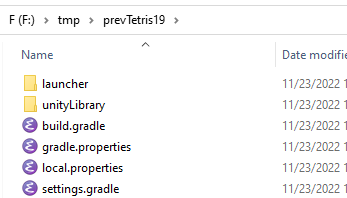
\includegraphics[width=.9\linewidth]{./pic/unityToAndroid_20221123_222322.png}
\begin{itemize}
\item 下面是2019年的版本可以打出两个文件夹,一个主工程,一个类库的导出包,2017年我用的版本打不出来,还需要想得再深一点多点儿,到可以按照这个笔记过程打包才行
\item 原始自己参考的项目是用2017版本的,当时没有吃透这里面的构建关系,当时以为只能用2017的unity和2017的Visual Studio才能开发.现在知道2019的版本能够导出自己可以调试的Android Studio项目,而unity 2017版本的导出来自己还仍不知道该如何从Android Studio打包,那么就暂时先用2019的版本,先试图打出在安卓设备上可运行的包,才能move on.
\end{itemize}

\section{Android  启动运行 unity}
\label{sec-5}
\subsection{在unity的AndroidMainfest.xml文件}
\label{sec-5-1}
\begin{itemize}
\item 把<intent-filter>-->删掉或者注释掉,留着的话,当我们把程序运行到手机或者模拟机上时会有两个图标。
\item 其次是在<activity>里加入这行代码,实现多线程,避免在从unity返回Android时也将Android界面也结束了。
\begin{minted}[fontsize=\scriptsize,linenos=false]{xml}
android:process=":raadidcard"
\end{minted}
\end{itemize}

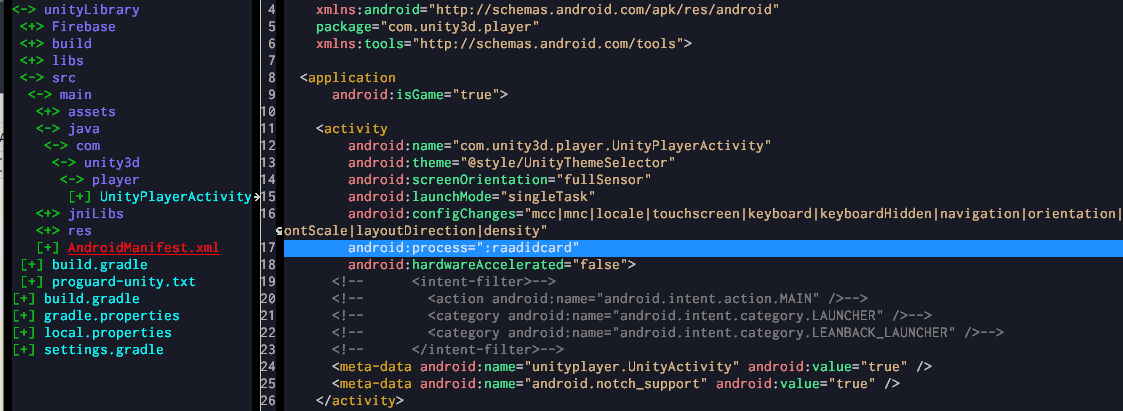
\includegraphics[width=.9\linewidth]{./pic/unityToAndroid_20221123_223227.png}
\subsection{在app的AndroidMainfest.xml文件里,在图中位置加入这两行代码:}
\label{sec-5-2}
\begin{minted}[fontsize=\scriptsize,linenos=false]{xml}
xmlns:tools="http://schemas.android.com/tools"

tools:replace="android:icon,android:theme,android:allowBackup"
\end{minted}
\begin{itemize}
\item 可以成片复制的代码如下:
\begin{minted}[fontsize=\scriptsize,linenos=false]{xml}
<?xml version="1.0" encoding="utf-8"?>
<manifest xmlns:android="http://schemas.android.com/apk/res/android"
          xmlns:tools="http://schemas.android.com/tools"
          package="com.unity3d.player">

  <application
      android:allowBackup="true"
      android:dataExtractionRules="@xml/data_extraction_rules"
      android:fullBackupContent="@xml/backup_rules"
      android:icon="@mipmap/ic_launcher"
      android:label="@string/app_name"
      android:roundIcon="@mipmap/ic_launcher_round"
      android:supportsRtl="true"
      tools:replace="android:icon,android:theme,android:allowBackup"
      android:theme="@style/Theme.Test"
      tools:targetApi="31">

    <activity
        android:name=".MainActivity"
        android:exported="true">
      <intent-filter>
        <action android:name="android.intent.action.MAIN" />
        <category android:name="android.intent.category.LAUNCHER" />
      </intent-filter>
      <meta-data
          android:name="android.app.lib_name"
          android:value="" />
    </activity>

  </application>
</manifest>
\end{minted}
\end{itemize}

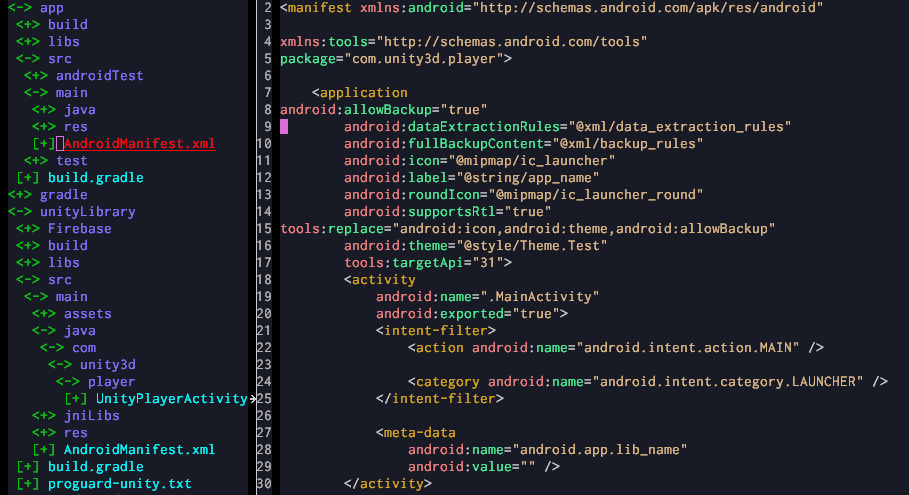
\includegraphics[width=.9\linewidth]{./pic/unityToAndroid_20221123_223757.png}

\subsection{在app的build.gradle里加入这行代码。}
\label{sec-5-3}
\begin{minted}[fontsize=\scriptsize,linenos=false]{xml}
ndk {
    abiFilters 'armeabi-v7a'
}
\end{minted}

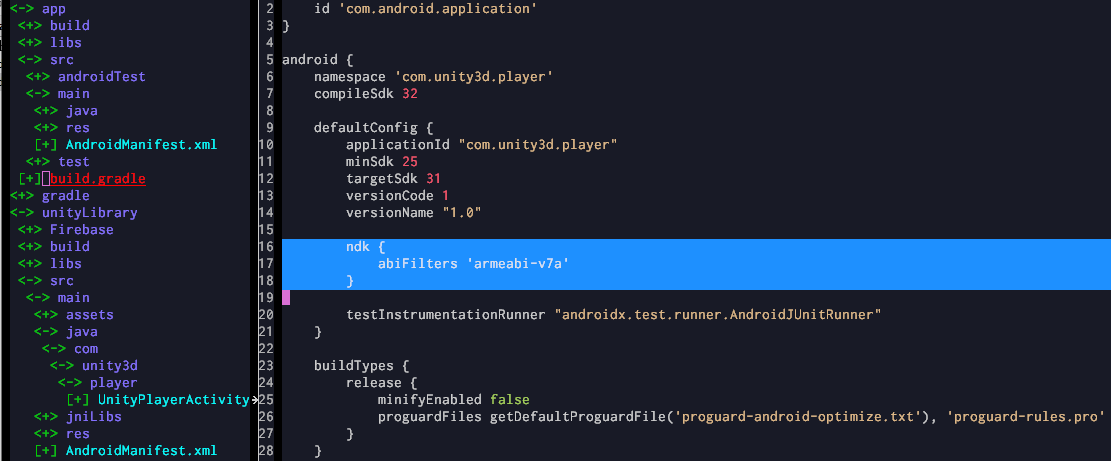
\includegraphics[width=.9\linewidth]{./pic/unityToAndroid_20221123_223842.png}
\subsection{在app的main->res->values->strings.xml里加入这行代码}
\label{sec-5-4}
\begin{itemize}
\item 都还没有去想,这句话能起到什么作用,应该是关系不大,或是可以跳过绕过的小细节
\begin{minted}[fontsize=\scriptsize,linenos=false]{xml}
<string name="game_view_content_description">Game view</string>
\end{minted}
\item 进行这两步操作的原因是,我在运行到手机时,他显示硬件不支持或者闪退。加入上面两个代码后就可以正常启动unity。
\item 我个人认为真正起作用的是上上一步关于手机架构的设置的ndk那三行,与上面字符串无关,应该是无关的
\end{itemize}

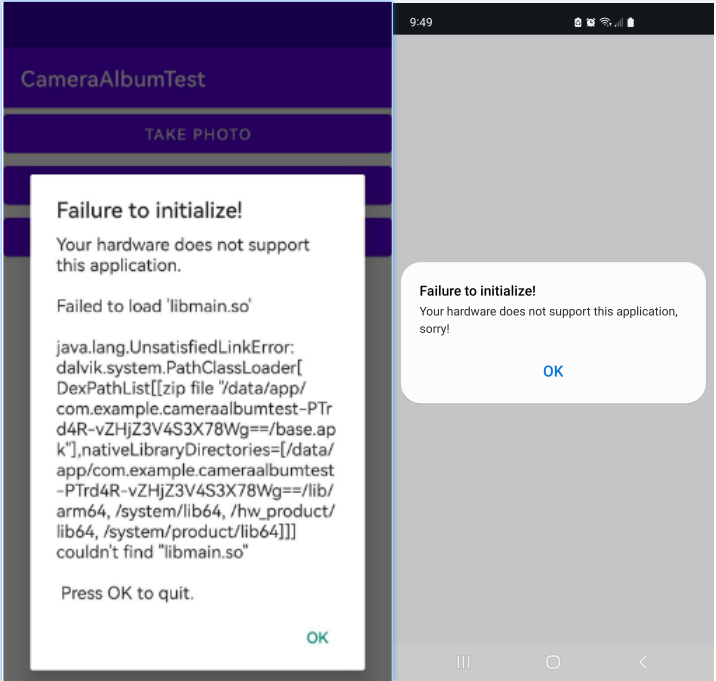
\includegraphics[width=.9\linewidth]{./pic/unityToAndroid_20221123_225409.png}

\subsection{点击按钮启动unity(画蛇添足)}
\label{sec-5-5}
\begin{itemize}
\item 感觉这个连接过程对于自己的项目就是画蛇添足.可是如何既能避开这一步,又能两者很好的平滑交互呢? 对于现在的自己,是个问题和挑战
\item 在主工程的activity\_main.xml 文件里添加一个按钮。MainActivity.java 里加入启动事件,如果在这里layout标红的话,就把鼠标移到layout下面,建立一个layout就行,我分析是主工程的问题,这个影响不大
\end{itemize}
\begin{minted}[fontsize=\scriptsize,linenos=false]{xml}
<Button
    android:id="@+id/showUnityBtn"
    android:layout_width="match_parent"
    android:layout_height="wrap_content"
    android:text="Show Unity"/>
\end{minted}

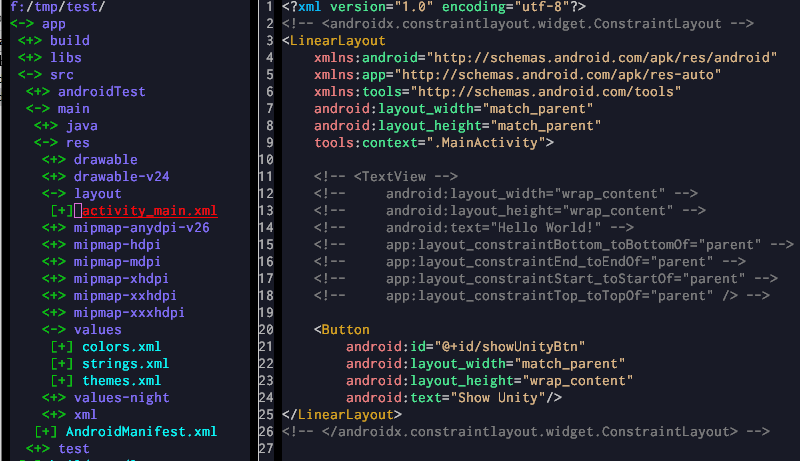
\includegraphics[width=.9\linewidth]{./pic/unityToAndroid_20221123_223751.png}
\begin{itemize}
\item MainActivity.cs 里的回调设置
\end{itemize}
\begin{minted}[fontsize=\scriptsize,linenos=false]{java}
Button btn = (Button)findViewById(R.id.showUnityBtn);
btn.setOnClickListener(new View.OnClickListener() {
        @Override
        public void onClick(View view) {

// <<<<<<<<<<<<<<<<<<<< UnityPlayerActivity <= com.unity3d.player 这里就是刚刚那个包名奇怪的地方,要不然 找不到 下面的 UnityPlayerActivity 类
            Intent intent = new Intent(MainActivity.this, UnityPlayerActivity.class); // <<<<<<<<<<<<<<<<<<<< UnityPlayerActivity

            startActivity(intent);
        }
    });
\end{minted}

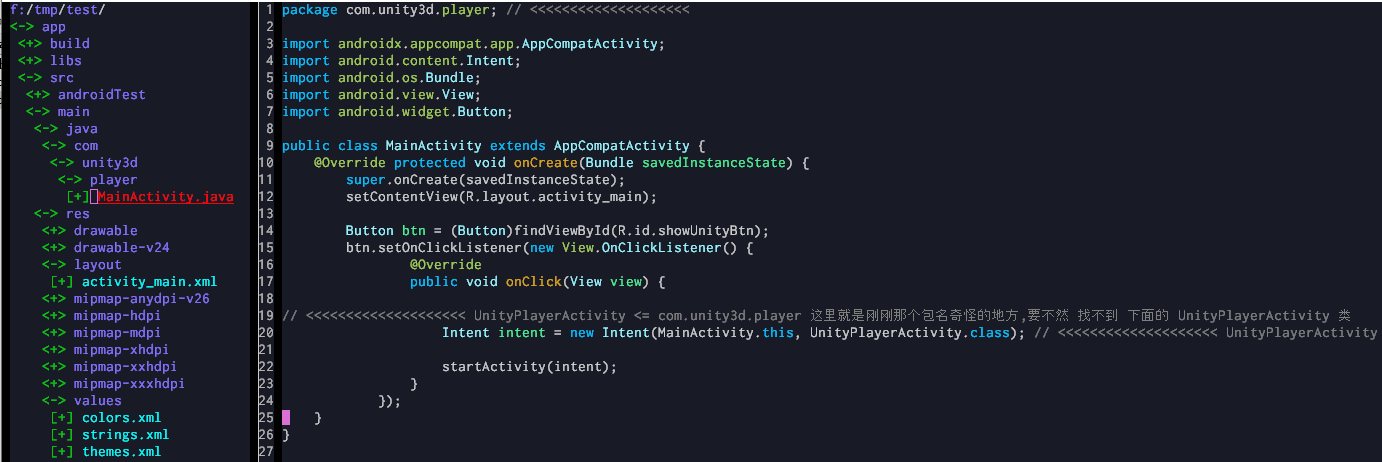
\includegraphics[width=.9\linewidth]{./pic/unityToAndroid_20221123_223852.png}
\subsection{在build.gradle中申明包裹类名称}
\label{sec-5-6}
\begin{itemize}
\item 说是现在在AndroidManifest.xml里申明包裹名称已经过时了,要在配置文件里申明,于是我在这里申明的:
\end{itemize}
\begin{minted}[fontsize=\scriptsize,linenos=false]{groovy}
android {
    namespace 'com.unity3d.player'
}
\end{minted}

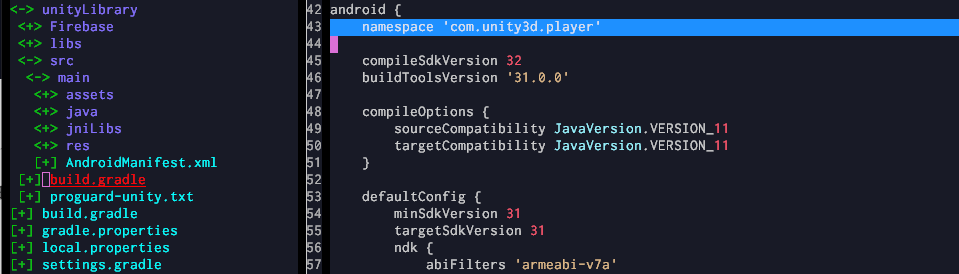
\includegraphics[width=.9\linewidth]{./pic/unityToAndroid_20221124_090438.png}

\section{启动运行}
\label{sec-6}

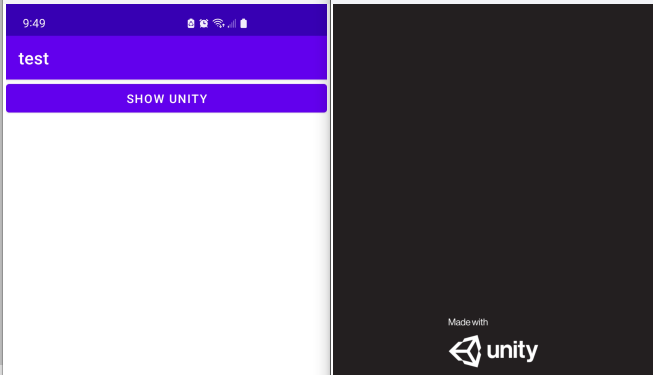
\includegraphics[width=.9\linewidth]{./pic/unityToAndroid_20221123_225517.png}

\section{Android Studio 类库中重复类的修复}
\label{sec-7}

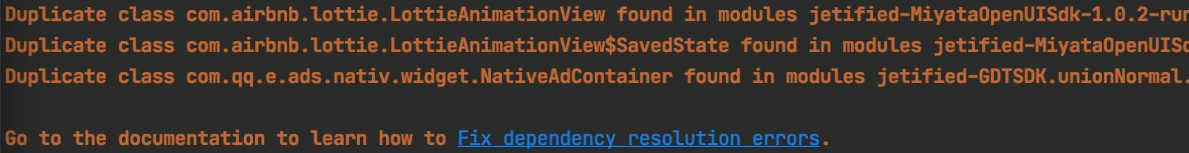
\includegraphics[width=.9\linewidth]{./pic/unityToAndroid_20221124_221720.png}
\begin{itemize}
\item 如果新导入的依赖库发生了 Duplicate class android.xx.xx 这种类型的报错可能就是两个库导入了重复的类,这时候只需要把build.gradle中新导入的依赖做如下处理
\begin{minted}[fontsize=\scriptsize,linenos=false]{xml}
implementation ('com.xxx.xxx.xx:xx:1.0.0'){
    exclude group: "com.xxxx.xxxx"
}
\end{minted}
\item 上面这个方法我还没有试.下面的试过了可行
\item 对,就是把新导入的依赖库的后面加上大括号并把重复导入包名填入相应的位置就可以解决了,有时候可能会好几个依赖库都重复了,这就比较难判断了
\item 1.把MiyataOpenUISdk-1.0.2.aar改后缀成zip,得到解压后的MiyataOpenUISdk-1.0.2文件夹,里面包含classes.jar和res等。
\end{itemize}

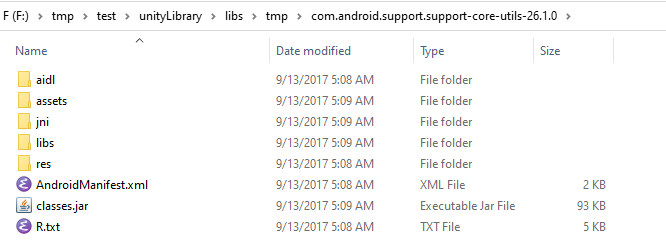
\includegraphics[width=.9\linewidth]{./pic/unityToAndroid_20221124_221954.png}
\begin{itemize}
\item 2.同理把classes.jar改后缀成zip,解压后得到classes文件夹,找到冲突的包,直接删除整个文件夹,如图
\item 3.使用jar命令重新对classes文件夹打包成jar ,并替换掉之前的classes.jar。
\end{itemize}
\begin{minted}[fontsize=\scriptsize,linenos=false]{shell}
jar cvf classes.jar -C classes/ .
\end{minted}
\begin{itemize}
\item 4.同理,使用jar命令重新对MiyataOpenUISdk-1.0.2文件夹打包成aar ,得到的newMiyataOpenUISdk.aar即可使用。
\end{itemize}
\begin{minted}[fontsize=\scriptsize,linenos=false]{shell}
 jar cvf com.android.support.support-compat-26.1.0.aar -C com.android.support.support-compat-26.1.0/ .
\end{minted}

\section{安卓Android Studio库包中有依赖的库包的解决方案 7.2.2}
\label{sec-8}
\begin{minted}[fontsize=\scriptsize,linenos=false]{tex}
Direct local .aar file dependencies are not supported when building an AAR.
\end{minted}
\begin{itemize}
\item 在高版本的AndroidStudio并且使用了版本的gradle出现了上述问题可以按着如下引用
\end{itemize}
\subsection{比较好一点的,是如下:在项目的根目录的build.gradle里申明类库unityLibrary的依赖的文件路径就可找到}
\label{sec-8-1}
\begin{minted}[fontsize=\scriptsize,linenos=false]{xml}
allprojects {
  buildscript {
      repositories {
          google()
          jcenter()
      }

      dependencies {
          classpath 'com.android.tools.build:gradle:7.2.2'
      }
  }

  repositories {
      google()
      jcenter()
     flatDir {
         dirs "${project(':unityLibrary').projectDir}/libs"
     }
  }
}

task clean(type: Delete) {
  delete rootProject.buildDir
}
\end{minted}

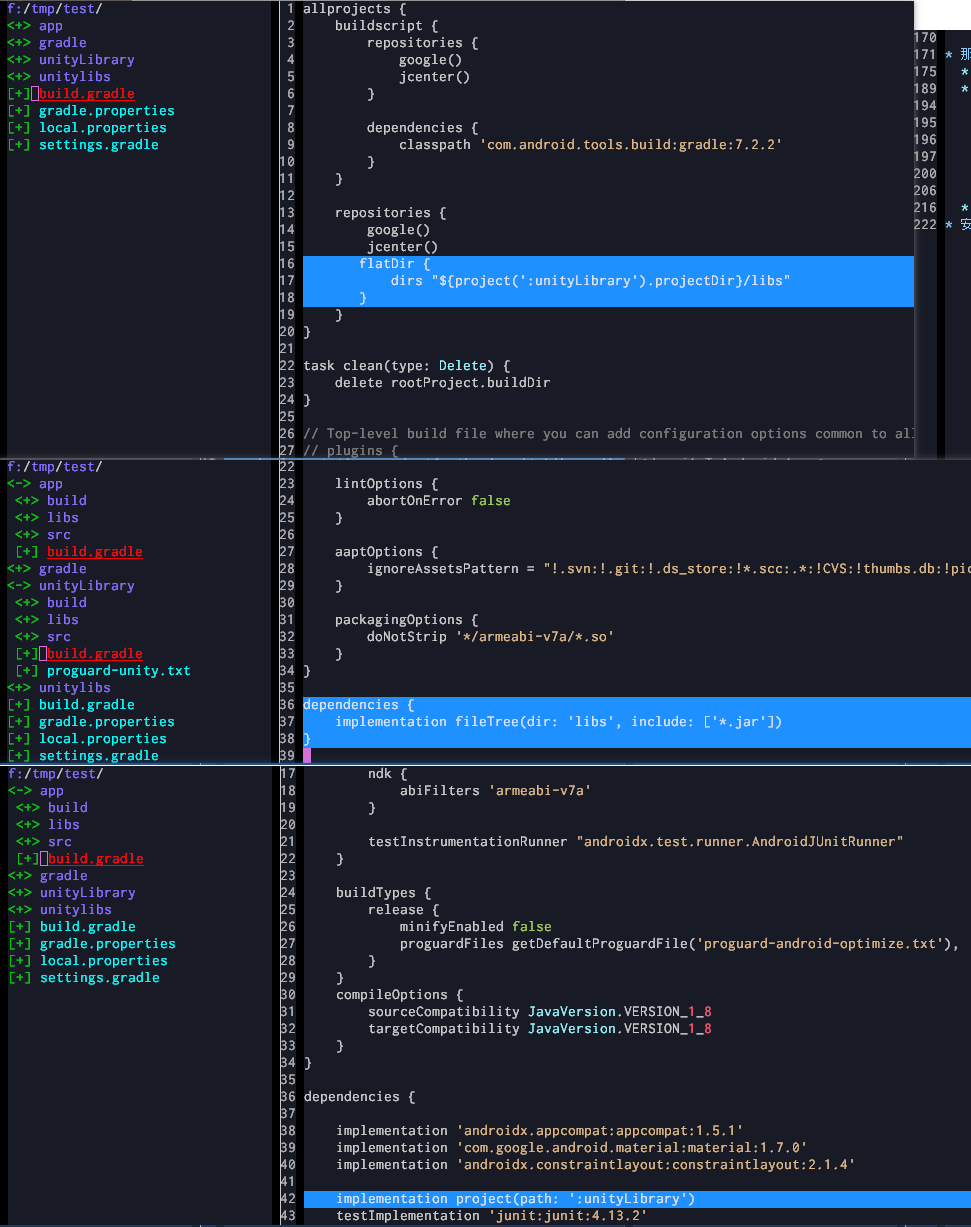
\includegraphics[width=.9\linewidth]{./pic/unityToAndroid_20221125_144439.png}

\subsection{下面的只是一种解决方案,可能还不是很好}
\label{sec-8-2}
\subsection{在你工程根目录下新建一个文件夹 \textbf{unitylibs} ,将你的aar文件放入,然后在该目录下新建一个build.gradle文件}
\label{sec-8-3}

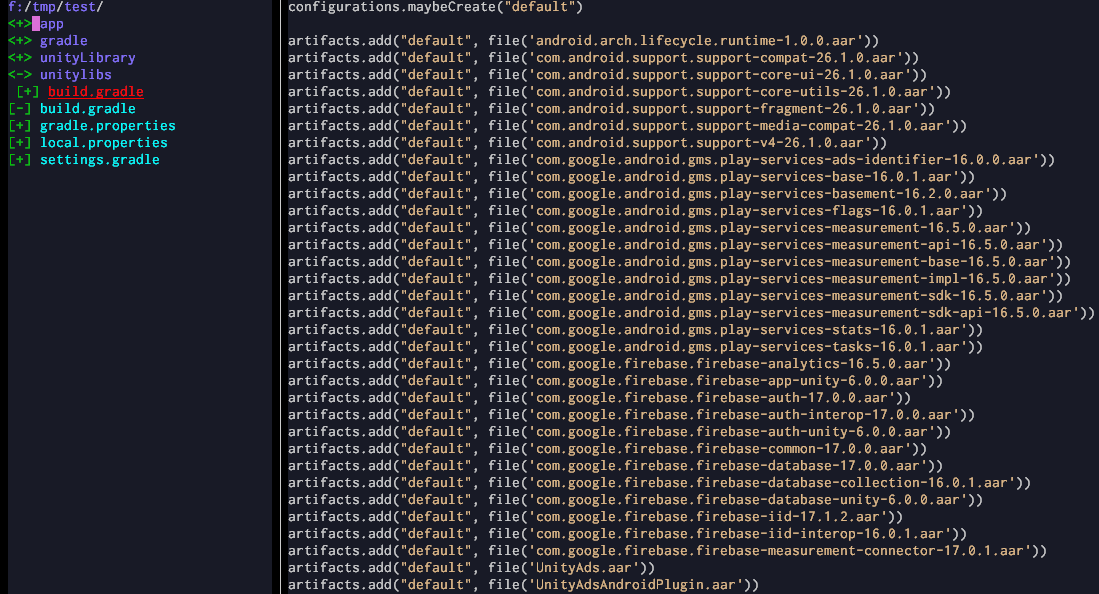
\includegraphics[width=.9\linewidth]{./pic/unityToAndroid_20221124_161335.png}
\subsection{在settings.gradle 导入该工程}
\label{sec-8-4}
\begin{minted}[fontsize=\scriptsize,linenos=false]{xml}
include ':unitylibs
\end{minted}

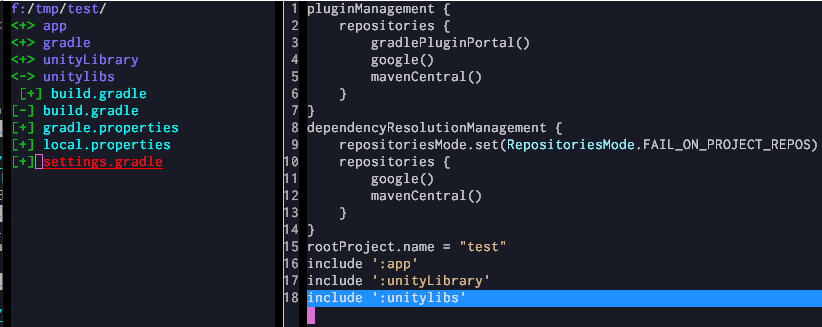
\includegraphics[width=.9\linewidth]{./pic/unityToAndroid_20221124_161424.png}
\subsection{在你需要依赖的工程里面的build.gradle中增加依赖}
\label{sec-8-5}
\begin{itemize}
\item // 这里需要注意的是,unitylibs是你aar库所在文件夹
\begin{minted}[fontsize=\scriptsize,linenos=false]{xml}
implementation project(path: ':unitylibs')
\end{minted}
\end{itemize}

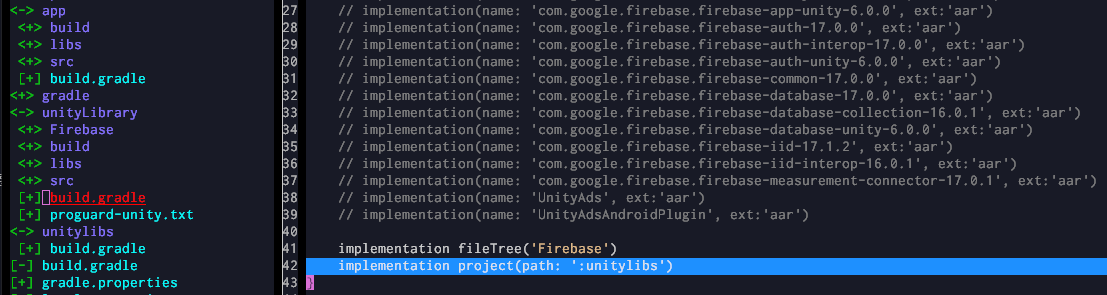
\includegraphics[width=.9\linewidth]{./pic/unityToAndroid_20221124_162337.png}
\begin{itemize}
\item 当然如果你有很多aar库,那么你需要在根目录创建一个LocalRepo目录,然后将你不同的aar库放在不同文件夹下。在setting.gradle分别导入
\item 下面它是这么说的,可是我都把它们放在同一个类库里,看不行的话再移.为什么每个包都需要一个单独的类库呢?解偶多个不同包之间的依赖性?加载时的内存性能影响等?
\end{itemize}

\section{安卓设备上资源包的存放位置,以及是否本地存放有需要的资源包}
\label{sec-9}
\begin{minted}[fontsize=\scriptsize,linenos=false]{text}
This PC\HEYAN's S10+\Internal storage\Android\data\com.defaultcompany.trunk\files
\end{minted}

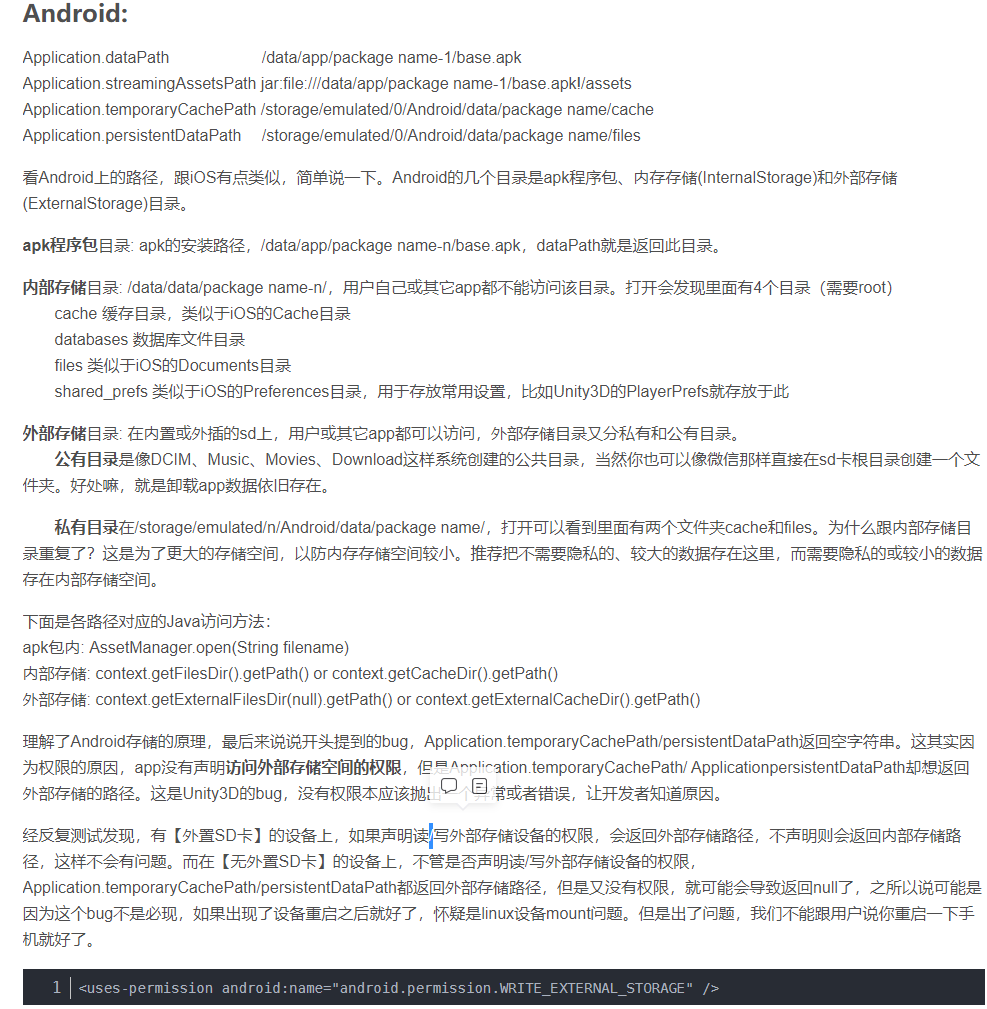
\includegraphics[width=.9\linewidth]{./pic/unityToAndroid_20221124_135846.png}

\begin{minted}[fontsize=\scriptsize,linenos=false]{tex}
Application.dataPath             /data/app/package name-1/base.apk
Application.streamingAssetsPath jar:file:///data/app/package name-1/base.apk!/assets
Application.temporaryCachePath  /storage/emulated/0/Android/data/package name/cache
Application.persistentDataPath  /storage/emulated/0/Android/data/package name/files
\end{minted}
\begin{itemize}
\item 看Android上的路径,跟iOS有点类似,简单说一下。Android的几个目录是apk程序包、内存存储(InternalStorage)和外部存储(ExternalStorage)目录。
\item \textbf{apk程序包目录}: apk的安装路径,/data/app/package name-n/base.apk,dataPath就是返回此目录。
\item \textbf{内部存储目录}: /data/data/package name-n/,用户自己或其它app都不能访问该目录。打开会发现里面有4个目录(需要root)
\item     cache 缓存目录,类似于iOS的Cache目录
\item     databases 数据库文件目录
\item     files 类似于iOS的Documents目录
\item     shared\_prefs 类似于iOS的Preferences目录,用于存放常用设置,比如Unity3D的PlayerPrefs就存放于此
\item 外部存储目录: 在内置或外插的sd上,用户或其它app都可以访问,外部存储目录又分私有和公有目录。
\item     公有目录是像DCIM、Music、Movies、Download这样系统创建的公共目录,当然你也可以像微信那样直接在sd卡根目录创建一个文件夹。好处嘛,就是卸载app数据依旧存在。
\item     私有目录在/storage/emulated/n/Android/data/package name/,打开可以看到里面有两个文件夹cache和files。为什么跟内部存储目录重复了?这是为了更大的存储空间,以防内存存储空间较小。推荐把不需要隐私的、较大的数据存在这里,而需要隐私的或较小的数据存在内部存储空间。
\item 下面是各路径对应的Java访问方法:
\begin{itemize}
\item apk包内: AssetManager.open(String filename)
\item 内部存储: context.getFilesDir().getPath() or context.getCacheDir().getPath()
\item 外部存储: context.getExternalFilesDir(null).getPath() or context.getExternalCacheDir().getPath()
\end{itemize}
\end{itemize}
理解了Android存储的原理,最后来说说开头提到的bug,Application.temporaryCachePath/persistentDataPath返回空字符串。这其实因为权限的原因,app没有声明访问外部存储空间的权限,但是Application.temporaryCachePath/ ApplicationpersistentDataPath却想返回外部存储的路径。这是Unity3D的bug,没有权限本应该抛出一个异常或者错误,让开发者知道原因。
\begin{itemize}
\item 经反复测试发现,有【外置SD卡】的设备上,如果声明读/写外部存储设备的权限,会返回外部存储路径,不声明则会返回内部存储路径,这样不会有问题。而在【无外置SD卡】的设备上,不管是否声明读/写外部存储设备的权限,Application.temporaryCachePath/persistentDataPath都返回外部存储路径,但是又没有权限,就可能会导致返回null了,之所以说可能是因为这个bug不是必现,如果出现了设备重启之后就好了,怀疑是linux设备mount问题。但是出了问题,我们不能跟用户说你重启一下手机就好了。
\end{itemize}
\begin{minted}[fontsize=\scriptsize,linenos=false]{xml}
<uses-permission android:name="android.permission.WRITE_EXTERNAL_STORAGE"/>
\end{minted}

\section{那么现在就是说:安卓SDK与unity的交互与打包基本没有问题了}
\label{sec-10}
\begin{itemize}
\item This PC\HEYAN's S10+\Internal storage\Android\data\com.defaultcompany.trunk\files
\end{itemize}

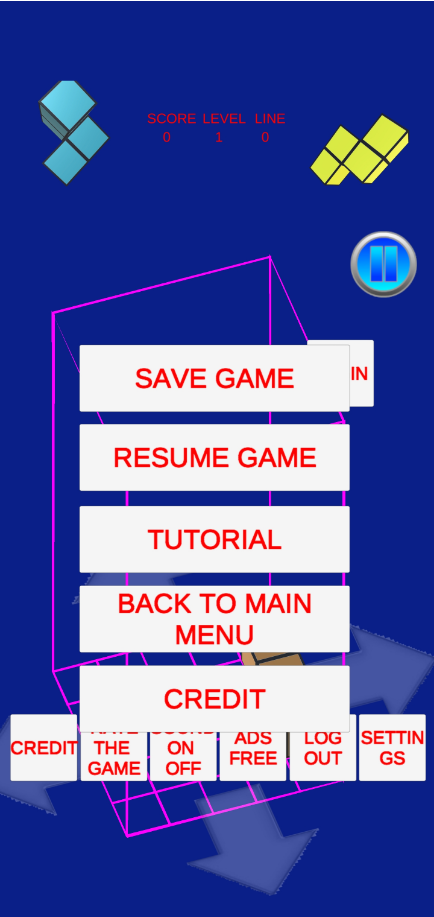
\includegraphics[width=.9\linewidth]{./pic/unityToAndroid_20221125_171932.png}

\begin{itemize}
\item 但对自己更大的挑战是:为什么unity里一个空物件挂载到热更新的过程,我打包之后在安卓手机上运行不出来,仍需要时间debug这个过程(呵呵,前面昨天还是前天已经想到问题的原因,不到因为探讨其它的想法,直到今天傍晚刚才整个过程才理通.不过目前仍是用unity直接到包,还有许多其它的细节小问题需要解决)
\item 过程中遇到过,还会遇到很多不懂的问题,比如同样的某些android studio里加android:exported="true"各种标签等,如果只用unity打包,该如何实现呢?两套不同的打包机制都得弄明白.但都是这么一个学习的过程,不会被轻易挫败.
\item 相比之下,安卓SDK的实现极其简单,可以放在后面
\end{itemize}
\subsection{FATAL EXCEPTION: main}
\label{sec-10-1}

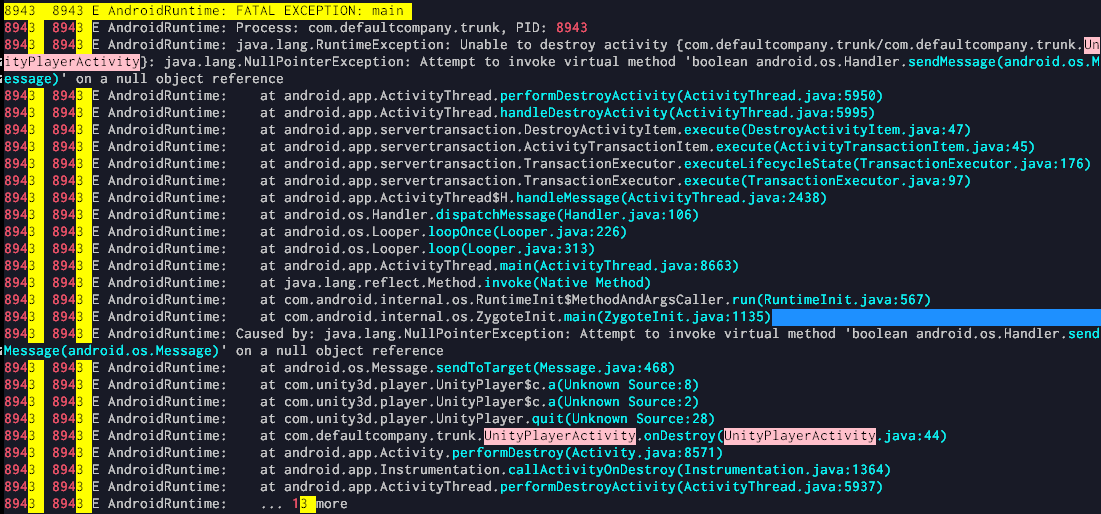
\includegraphics[width=.9\linewidth]{./pic/unityToAndroid_20221124_101807.png}
\begin{itemize}
\item 这个没有再出现了,根据这里改的:\url{https://forum.unity.com/threads/android-crashes-after-update-project-to-unity-2020-3-9f.1126979/}
\item 但是游戏的界面仍然是渲染不出来,还在找原因
\end{itemize}
\begin{minted}[fontsize=\scriptsize,linenos=false]{java}
@Override protected void onDestroy () {
    Log.d(TAG, "onDestroy() ");
    // mUnityPlayer.destroy();
    mUnityPlayer.removeAllViews();
    mUnityPlayer.quit();
    super.onDestroy();
}
\end{minted}
\subsection{类库包里的错误的修复问题}
\label{sec-10-2}
\begin{itemize}
\item 现在还不是很懂,或是还没有经历狠好地锻炼怎么改类库包里的错误,晚点儿再理会这些
\end{itemize}

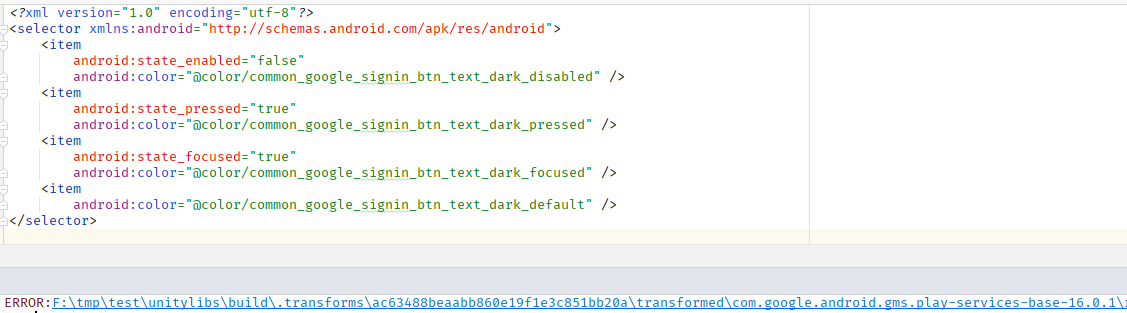
\includegraphics[width=.9\linewidth]{./pic/unityToAndroid_20221124_163004.png}
\begin{itemize}
\item 先只把这些有错误的类库包不连上
\end{itemize}
% Emacs 27.2 (Org mode 8.2.7c)
\end{document}